% book example for classicthesis.sty
\documentclass[11pt,a5paper,footinclude=true,headinclude=true]{report} % KOMA-Script book
\usepackage[T1]{fontenc}                
\usepackage[linedheaders,parts,pdfspacing]{classicthesis} % ,manychapters
%\usepackage[osf]{libertine}
\usepackage{amsthm}
\usepackage{graphicx}
\usepackage[T1]{fontenc}
\newcommand{\HRule}{\rule{\linewidth}{0.5mm}}
\usepackage{float}
\RequirePackage{titletoc}


%%%%%%%%%%%%%%%%%%%%%%%%%%%%


%
\titlecontents{chapter}[1.3cm] % <-- seems to set some specific left margin
{\addvspace{3mm}}
{\makebox[0cm][r]{\large\bf\hspace{.0em}\thecontentslabel\hspace{.75cm}}}
{} %     ^^^ pretendously zero width box puts its contents in the left margin
{\hfill\makebox[-3cm]{\thecontentspage}}  % 3cm
%%
\titlecontents{section}[2cm] % <-- again this left (additional?) margin
{\addvspace{3mm}}
{\makebox[0cm][r]{\thecontentslabel\hspace{.75cm}}} % box pushed to the left
{}
{\hfill\makebox[-3cm]{\thecontentspage}}  % 3cm = twice 1.5cm
[\addvspace{0mm}]

%%%%%%%%%%%%%%%%%%%%%%%%


\begin{document}
\begin{titlepage}
    \begin{center}
        \vspace*{1cm}
        
 
        \HRule \\[0.4cm]
        {   \huge\textbf{Software Requirements and Specifications}\\[0.4cm] }
        \HRule \\[1cm]
       
        
        \vspace{0.5cm}
        \LARGE
        Thesis Subtitle
        
        \vspace{1.5cm}
        
        \textbf{The A-Team}
        
        \vfill
        
        A thesis presented for the degree of\\
        Doctor of Philosophy
        
        \vspace{0.8cm}
        
        
\includegraphics[width=0.4\textwidth]{UMASS_logo}
        
        \Large
        Department Name\\
        University Name\\
        Country\\
        Date
        
    \end{center}
\end{titlepage}
	\tableofcontents 
	
	%INTRO
\part{Introduction}
\chapter {System Overview}

The purpose of this system is to be an online tutor for students who are learning to create ER diagrams. This learning tool teaches students to build ER diagrams and allows them to submit the diagrams that they create as responses to assignment questions. The assignments are created by instructors using questions that are taken from the question bank. Each question, that is stored in 
the question bank, is created by an author and includes any correct answers and necessary feedback that correspond to it. After a student submits a diagram to be graded, he or she is either notified that diagram is correct or given feedback about the incorrectness of the diagram. This allows each student to learn from his or her mistakes. Overall, the benefits of this system are that it serves as an easier and more efficient tool for students who are learning to create ER diagrams and submitting assignments and instructors who are creating assignments and viewing student reports.  

\chapter{Stakeholders}
The stakeholders of the system involve the three defined user groups (authors, instructors and students), as well as the client, management, administrators, and developers. The administrators of the system will be involved in managing the three user groups. Administrators will give access rights to each group based on what they need to do (Authors can create questions, but instructors/students can$'$t, etc.). While the system itself has the capability to manage direct user registration the administrators have a stake in ensuring that the system is accessible to those who need it. The users all have a stake in either accessing, modifying, or creating the questions hosted within the system, and the question bank in general. The instructors who have access to the system have a stake in creating groups of questions for students and in a lesser sense creating or editing questions to their needs, and accessing reported student progress on those content clusters. Authors primarily add and edit questions in the bank and will not directly interface with student answers. Students do not create or edit questions, but answer and submit content clusters as assigned by instructors. The client and management have stakes in the system because they are responsible for providing guidance to ensure that the final product is what they want. Naturally, this leaves the developers to have a stake in the system by implementing the wants and needs of the client and management into the system.


\chapter{Scope of the Document}
This document describes the architectural layout of the online tutoring system. It includes an overview, stakeholders and a glossary to help define and describe the important system attributes. In addition, this document displays many design modules that come together to help form the architecture of the online tutoring system.  These design modules include a deployment design, which describes the technologies used for each component of the system, a  modular design, which describes the different client and server modules that are involved in transferring data, a client design, which describes all of the methods that are responsible for performing different client actions, and a server design, which describes the server$'$s role as the connection between the client and the data base.     


\chapter{Definitions}
\begin{itemize}
\item The online tutor system is the system that is being created in order to facilitate the instruction and education of constructing ER diagrams.
\item A student is a user that is accessing the online tutor system in order to learn and practice making ER diagrams.
\item The learning tool is the system that is used by a student to understand how to create ER diagrams.
An assignment is a collection of questions that the instructor selects for students to answer by a certain date.
\item Each student report, for a particular assignment, displays a unique student$'$s results to that assignment.
\item The instructor is the user who creates assignments by selecting questions from the question bank for students to answer. Also, the instructor can view the student reports for each assignment.
\item Feedback is the message that is returned to each student after he/she submits an answer. It can be composed of hints, suggestions and messages from the author.
The author is the user who creates the questions, answers and feedback. Also, the author uploads those questions, answers and feedback to the question bank for instructors to use when creating assignments.
\item Draw is the action that students or author performs to insert the shapes and words from the toolbox to the answer area of the UI. This action occurs when students are answering questions or when the author is creating answers to questions.
\item A question is created by an author (for an instructor to pull from the question bank), assigned by an instructor (in an assignment) and answered by a student (with an ER diagram).
\item  The toolbox is the area of the UI that contains all of the shapes, lines and textboxes for the user or author to drag and drop onto the draw space when drawing.
\item An answer is created by an author (with a corresponding question) and constructed by a student (in the form of an ER diagram) to respond to an assigned question. A student$'$s answer to a specific question in an assignment will be graded when that assignment is submitted.
\item NetID is the username that a user uses to log into the system.
\item Password is the password that a user uses to log into the system.
\item The question bank is the database that contains all of the questions that have been created by the author. The instructor selects questions from the question bank to create assignments for students.
\item The draw space is the area in which the answer to a question is drawn.
\item The user is the person using the online tutoring system. There are three different types of users: students, instructors and authors.
\end{itemize}  
%DIAGRAMS
\part{Diagrams}
\chapter{Deployment Design}
      In this high-level deployment diagram, we show the technologies used for each component of the system. The client will use HTML, CSS, and JS, and will be run on the user$'$s machine. This will communicated with the server, which will be built with Nodejs and will run on a Unix system. These components will use a Postgres Database in order to store all of the information of the system (user results, assignments, etc.). The database will be on the same machine as the server.
                        \begin{figure}[H]
            \centerline{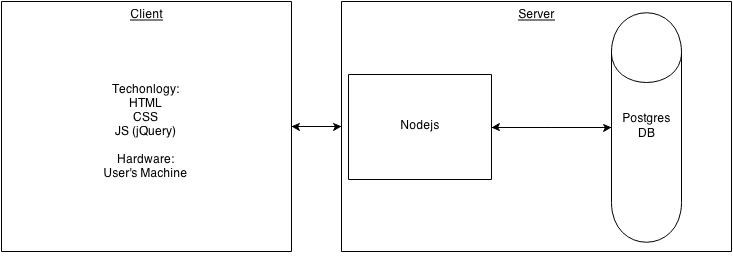
\includegraphics[height=3cm, width=10cm]{Deployment.jpg}}
            \caption{Deployment Diagram}
    \end{figure}
    
\chapter{Modular Design}
In this more detailed architecture design you can see the different modules in both the client and server sides.  The Client is made up of the Drawing Widget, Report Formatter, and Serializer while the Server is made up of the Deserializer, Dispatcher, Validator, DB Accessor and the DB.  The Drawing Widget contains everything needed for the user, author or student, to draw out either the question, answer or solution to a question that is displayed on the screen.  The Report Formatter is only used by the instructor user and takes the information that it receives from the database to compile a report on the students for the instructor to view.  The Serializer, is used for packaging and submitting the question and answer from the user to the server through http sending as a JSON.  The Deserializer is used to take what was sent from the server and undo the serialization that was used when sending information to the server.  On the Server side, the Dispatcher takes the information from the Server and packages the information to be sent to the client side of the system.  The Validator is used when a student submits an answer to a question to check the answer for correctness, and generate feedback to the student.  The DB Accessor is responsible for handling all of the requests made to send or receive information from the database.  Finally the DB is the database that contains the question bank, the student responses and assignments.    
 
                        \begin{figure}[H]
            \centerline{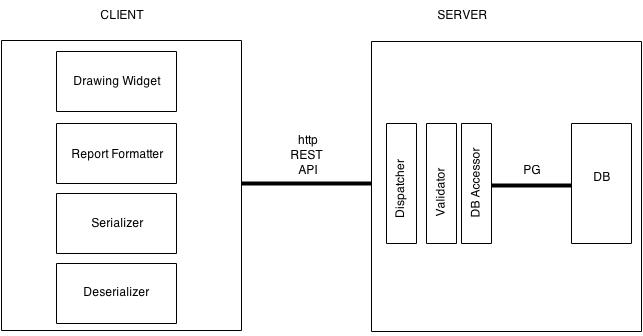
\includegraphics[height=5cm, width=10cm]{Modular.jpg}}
            \caption{Modular Diagram}
    \end{figure}
    
    \chapter{Client}
This is the diagram for the Client module. The following are the methods contained in it. openAssignment() is used by both students and instructors to open an assignment. It calls sendPageRequest() and renderPage() to render the page. createAssignment() is used by an instructor to create an assignment. openQuestion() is used by all three users, the authors, the instructors, and the students to open a question. It uses the render methods to render the page. The createQuestion() method is used by an author to create a question. drawDiagram() is used by both authors when creating the diagram and students when answering it. It uses the methods in DrawingWidget. placeEntity() to place the entities in the diagram, placeRelation() to place the relations in the diagram, and addText() to add text to the diagram. submitAnswer() is used to submit a diagram and calls sendToSerial() in DrawingWidget which uses the Serializer methods createSerialJSON() to convert the diagram into a JSON format, and sendJSON() to send this JSON to the server. openReport() is used by an instructor to view the student reports. The methods in ReportFormatter are used, collectStudentReports() retrieves the reports from the server, formatReports() formats the reports to be viewed, and render() renders the webpage.  When diagrams are sent back to the client from the server they go through the Deserializer which calls the methods, recieveJSON() when the JSON is passed back from the server and then unpackSerialJSON() to unpack the JSON back into a diagram.
  
                        \begin{figure}[H]
            \centerline{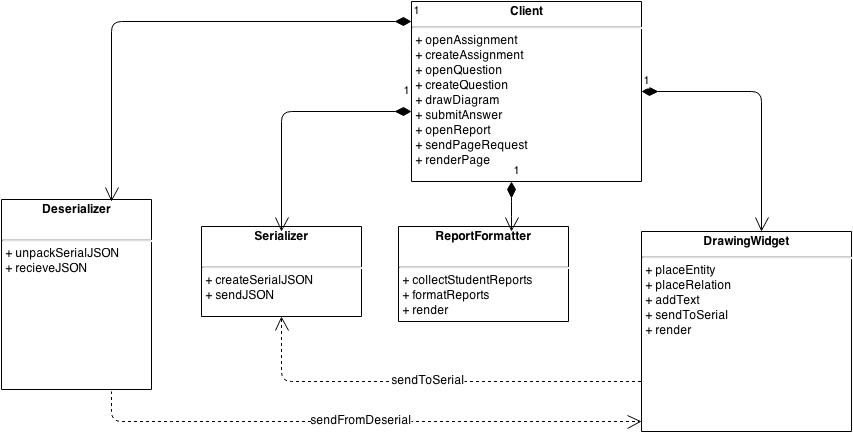
\includegraphics[height=5cm, width=10cm]{Client.jpg}}
            \caption{Client Diagram}
    \end{figure}
    
    \chapter{Server}
The server plays a huge role in our system, it is in charge of keeping connection with the Client and the database. The Dispatcher will process the question submitted by the user and request its validation with the validator. Then, the validator checks whether the question submitted by the student is actually correct or not, by going to the database accessor. Moreover, when the validator checks if a question is correct or not, it sends a customized feedback for that particular question.
The server also is able to update a particular question in the database that has been saved by the author. 

                        \begin{figure}[H]
            \centerline{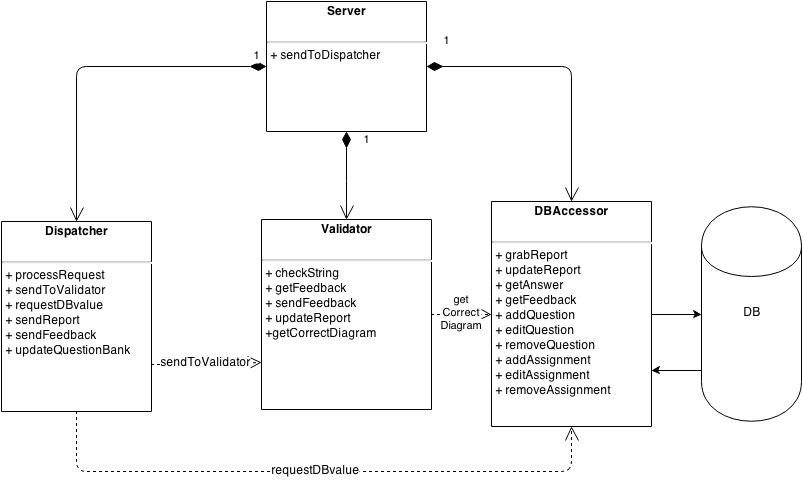
\includegraphics[height=4cm, width=10cm]{Server.jpg}}
            \caption{Server Diagram}
    \end{figure}
    


\part{Modules}
\chapter{Serializer}
\textbf{Description:} The serializer module provides a way for a client to send an ER diagram to the server by converting the ER diagram into a JSON. \\
\textbf{Interface Specification:}
\begin{itemize}
\item{JSON createSerialJSON(diagram) - This public method creates a JSON representation of an existing ER diagram.}
\item{void sendJSON() - This public method sends a JSON from a client to the server.}
\end{itemize}
\textbf{Assumptions:}
\begin{itemize}
\item{The ER diagram that is being used by this class is an existing and completed ER diagram.}
\end{itemize}
\textbf{Dependencies:}
This module is contained by the Client module and used by the DrawingWidget module. \\
\textbf{Internal Structure:}
\begin{itemize}
        	\item{\textbf{Internal Methods:} 
        	\begin{itemize}
        	\item{None}
        	\end{itemize}}
        	\item{\textbf{Internal Variables:} 
        	\begin{itemize}
        	\item{None}
        	\end{itemize}}
\end{itemize}
\textbf{Hidden Information:}
\begin{itemize}
\item{None}
\end{itemize}
 
\chapter{Deserializer}
\textbf{Description:} The deserializer module provides a way for a client to receive an ER diagram from a server by converting the JSON representation of an ER diagram back into the actual ER diagram. \\
\textbf{Interface Specification:}
\begin{itemize}
\item{diagram unpackSerialJSON() - This public method converts the JSON representation of an ER diagram back into the actual ER diagram.}
\item{JSON recieveJSON() - This public method allows a client to receive a JSON from the server.}
\end{itemize}
\textbf{Assumptions:}
\begin{itemize}
\item{The JSON that is being used by this class is the JSON representation of an existing and completed ER diagram.}
\end{itemize}
\textbf{Dependencies:}
This module is contained by the Client module and uses the DrawingWidget module. \\
\textbf{Internal Structure:}
\begin{itemize}
        	\item{\textbf{Internal Methods:} 
        	\begin{itemize}
        	\item{None}
        	\end{itemize}}
        	\item{\textbf{Internal Variables:} 
        	\begin{itemize}
        	\item{None}
        	\end{itemize}}
\end{itemize}
\textbf{Hidden Information:}
\begin{itemize}
\item{None}
\end{itemize}
 
\chapter{Dispatcher}
\textbf{Description:} The dispatcher takes the information from the Server and packages the information to be sent to the client side of the system. \\
\textbf{Interface Specifications:}
\begin{itemize}
\item{void processRequest - This public method processes the request to be sent to the database.}
\item{void sendToValidator - This public method sends a students answer to a question to the validator.}
\item{value requestDBValue -- This public method returns a value that is requested from the database through the DBAccessor module.}
\item{void sendReport -- This public method compiles and sends a report to the caller.}
\item{void sendFeedback -- This public method compilkes and sends feedback to the caller.}
\item{void updateQuestionBank -- This public method updates the question bank contained in the database.}
\end{itemize}
\textbf{Assumptions:}
\begin{itemize}
\item{The modules are online and accessible.} 
\end{itemize}
\textbf{Dependencies:}
This module is contained by the Server module and is dependent on the Validator module and DBAccessor module. \\
\textbf{Internal Structure:}
\begin{itemize}
        	\item{\textbf{Internal Methods:} 
        	\begin{itemize}
        	\item{None}
        	\end{itemize}}
        	\item{\textbf{Internal Variables:} 
        	\begin{itemize}
        	\item{None}
        	\end{itemize}}
\end{itemize}
\textbf{Hidden Information:}
\begin{itemize}
\item {None}
\end{itemize}


%MATT'S USE CASES:



\chapter{Toolbox}
\textbf{Description:} The Toolbox contains all of the different entities and relations that are possible for use in the ER Diagram.  The Toolbox has drag and drop capabilities to allow the user to click and then drag the desired entity or relation that they wish to insert into the Canvas to create the ER Diagram. \\
\textbf{Interface Specification:}
\begin{itemize}
\item{void selectEntity(entity) - this method is the user selecting an entity from the Toolbox and dragging it into the Canvas.}
\item{void selectRelation(relation) - this method is the user selecting a relation from the Toolbox and dragging it into the Canvas.}   
\item{List<entity> interactiveEntryList - variable that lists all of the possible entities in the Toolbox}
\item{List<relation> interactiveRelationList - variable that lists all of the possible relations in the Toolbox}
\end{itemize}
\textbf{Assumptions:} 
\begin{itemize}
\item {The Toolbox contains all of the possible entities and relations possible and the user can drag and drop them.}
\end{itemize}
\textbf{Dependencies:} This module is dependent on the DrawingWidget module, and Question module.  This module depends on the Entity module and the Relation module. \\ 
\textbf{Internal Structure:}
\begin{itemize}
        	\item{\textbf{Internal Methods:} 
        	\begin{itemize}
        	\item{None}
        	\end{itemize}}
        	\item{\textbf{Internal Variables:} 
        	\begin{itemize}
        	\item{None}
        	\end{itemize}}
\end{itemize}
\textbf{Hidden Information:}
\begin{itemize}
\item{None} 
\end{itemize}
 
\chapter{Relation}
\textbf{Description:} This module contains all of the relations or lines that connect the different entities.  There will be options for both Chen and Crows Foot styles of ER Diagrams.  The relations will show if it is many to one, one to many, one to one or many to many. \\
\textbf{Interface Specification:}
\begin{itemize}
\item{void addLabel(String) - Adding a description to the relation to describe the name and style of relation such as one to one, one to many, many to many, and many to one.}
\item{void relation(type) - creating a relation, the constructor of the class}
\item{Relation relation - the relation variable that is used in the class}
\end{itemize}
\textbf{Assumptions:}
\begin{itemize}
\item{All possible relations are present} 
\end{itemize}
\textbf{Dependencies:} This module is dependent on the Toolbox module and the DrawingWidget module.  It depends on the Entity module. \\
\textbf{Internal Structure:}
\begin{itemize}
        	\item{\textbf{Internal Methods:} 
        	\begin{itemize}
        	\item{None}
        	\end{itemize}}
        	\item{\textbf{Internal Variables:} 
        	\begin{itemize}
        	\item{String type - the type of relation}
        	\end{itemize}}
\end{itemize}
\textbf{Hidden Information:}
\begin{itemize}
\item{None} 
\end{itemize}

\chapter{Canvas}
\textbf{Description:} This module contains all the necessary components to build a graphical user interface. We want to ensure that all the components are well drawn and easy for the user to use. \\
\textbf{Interface Specification:}
\begin{itemize}
\item{deleteEntity(entity):void - deletes the specified entity}
\item{moveEntity(entity):void - moves the specified entity}
\item{deleteRelation(relation):void - deletes the specified relation}
\item{moveRelation(relation):void - moves the specified relation}
\end{itemize}
\textbf{Assumptions:}
\begin{itemize}
\item{None} 
\end{itemize}
\textbf{Dependencies: Canvas depends on the ToolBox and the DrawingWidget.}
\textbf{Internal Structure:}
\begin{itemize}
        	\item{\textbf{Internal Methods:} 
        	\begin{itemize}
        	\item{None}
        	\end{itemize}}
        	\item{\textbf{Internal Variables:} 
        	\begin{itemize}
        	\item{None}
        	\end{itemize}}
\end{itemize}
\textbf{Hidden Information:}
\begin{itemize}
\item{None} 
\end{itemize}

\chapter{DrawingWidget}
\textbf{Description:} This will contain everything needed in order to draw and view an ER diagram. This includes a Toolbox for selecting items to draw, and a Canvas to place the ER diagram. \\
\textbf{Interface Specification:}
\begin{itemize}
\item{Toolbox toolBox - Toolbox instance that will allow users to pick elements to draw}
\item{Canvas canvas - Canvas where the ER diagram will be drawn}
\end{itemize}
\textbf{Assumptions:}
\begin{itemize}
\item {None}
\end{itemize}
\textbf{Dependencies:} This module is dependent on the Toolbox and Canvas modules \\
\textbf{Internal Structure:}
\begin{itemize}
        	\item{\textbf{Internal Methods:} 
        	\begin{itemize}
        	\item{None}
        	\end{itemize}}
        	\item{\textbf{Internal Variables:} 
        	\begin{itemize}
        	\item{int size - size of the entire widget}
        	\end{itemize}}
\end{itemize}
\textbf{Hidden Information:}
\begin{itemize}
\item{None} 
\end{itemize}

\chapter{Entity}
\textbf{Description:} This module contains all the entities to be connected by relations in the ER diagram. There will be options for both Chen and Crows Foot styles of ER Diagrams. \\
\textbf{Interface Specification:}
\begin{itemize}
\item{void addText (String) - adding text to be placed inside of the entity.}
\item{void entity(type) - creating an entity, the constructor of the class.} 
\item{Entity entity - the entity variable that is used in the class.}
\end{itemize}
\textbf{Assumptions:}
\begin{itemize}
\item{All possible entities are present.}
\end{itemize}
\textbf{Dependencies:} This module is dependent on the Toolbox module and DrawingWidget module. It depends on the Relation module. \\
\textbf{Internal Structure:}
\begin{itemize}
        	\item{\textbf{Internal Methods:} 
        	\begin{itemize}
        	\item{None}
        	\end{itemize}}
        	\item{\textbf{Internal Variables:} 
        	\begin{itemize}
        	\item{String type - the type of entity}
        	\end{itemize}}
\end{itemize}
\textbf{Hidden Information:}
\begin{itemize}
\item{None} 
\end{itemize}







%%%%%%%%%%%%%%%%%%%%%%%%%%%%%%%%%%%%%%%%%%%%%%%%%%%%%%%%%%%
%%%%%%%%%%%%%%%%%%%%%UML%%%%%%%%%%%%%%%%%%%%%%%%%%%%%%%%%%%
%%%%%%%%%%%%%%%%%%%%%%%%%%%%%%%%%%%%%%%%%%%%%%%%%%%%%%%%%%%

\chapter{UML 3}

    \begin{figure}[H]
            \centerline{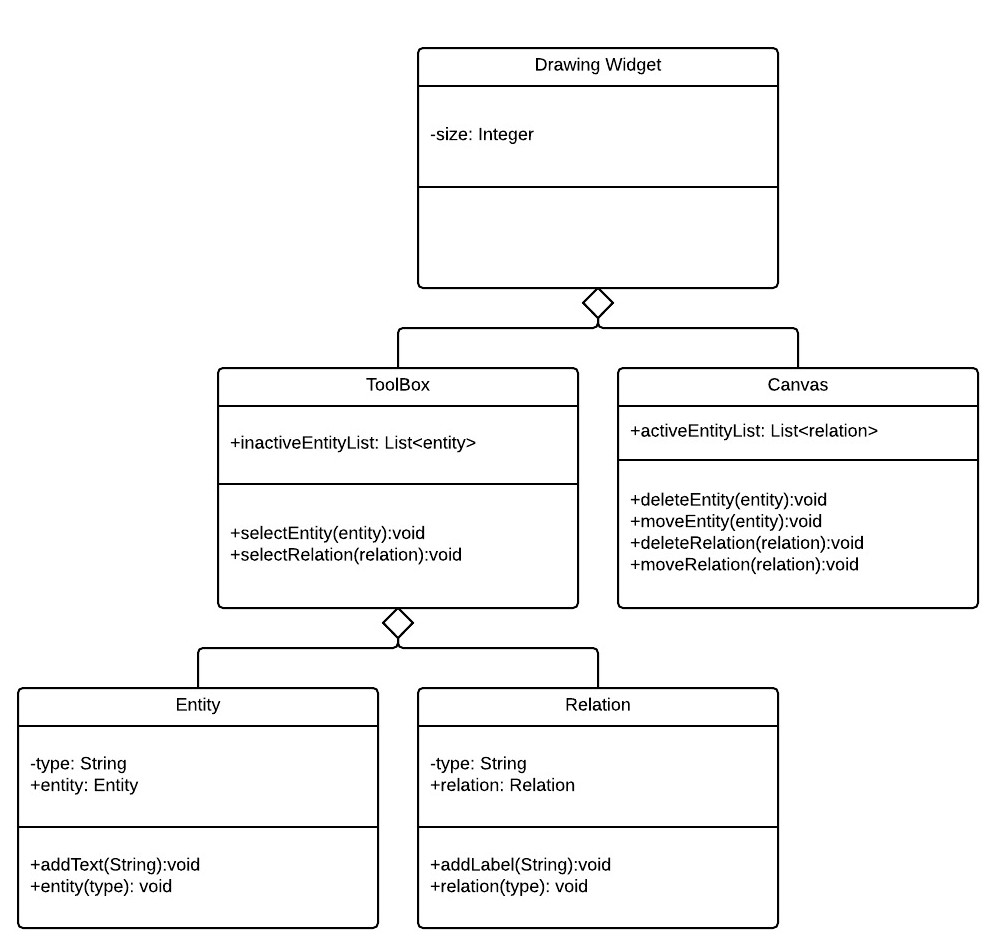
\includegraphics[height=9cm, width=10cm]{UML_3.jpeg}}
            \caption{UML3 Diagram}
    \end{figure}

%%%%%%%%%%%%%%%%%%%%%%%%%%%%%%%%%%%%%%%%%%%%%%%%%%%%%%%%%%%
%%%%%%%%%%%%%%%%%%%%%UML%%%%%%%%%%%%%%%%%%%%%%%%%%%%%%%%%%%
%%%%%%%%%%%%%%%%%%%%%%%%%%%%%%%%%%%%%%%%%%%%%%%%%%%%%%%%%%%
















\chapter{ReportFormatter}
\textbf{Description:} This module formats the student reports to be presented to an instructor. \\
\textbf{Interface Specification:}
\begin{itemize}
\item{void collectStudentReports() - collects the student reports from the database. }
\item{void formatReports() - formats the student reports to be readable.}
\item{void render() - renders the page and shows the student reports.}
\end{itemize}
\textbf{Assumptions:}
\begin{itemize}
\item{There are reports to format and present} 
\end{itemize}
\textbf{Dependencies:} This module is dependent on the DBAccessor module. \\ 
\textbf{Internal Structure:}
\begin{itemize}
        	\item{\textbf{Internal Methods:} 
        	\begin{itemize}
        	\item{None}
        	\end{itemize}}
        	\item{\textbf{Internal Variables:} 
        	\begin{itemize}
        	\item{None}
        	\end{itemize}}
\end{itemize}
\textbf{Hidden Information:}
\begin{itemize}
\item{None} 
\end{itemize}




%%%%%%%%%%%%%%%%%%%%%%%%%%%%%%%%%%%%%%%%%%%%%%%%%%%%%%%%%%%
%%%%%%%%%%%%%%%%%%%%%UML%%%%%%%%%%%%%%%%%%%%%%%%%%%%%%%%%%%
%%%%%%%%%%%%%%%%%%%%%%%%%%%%%%%%%%%%%%%%%%%%%%%%%%%%%%%%%%%

\chapter{UML 1}

    \begin{figure}[H]
            \centerline{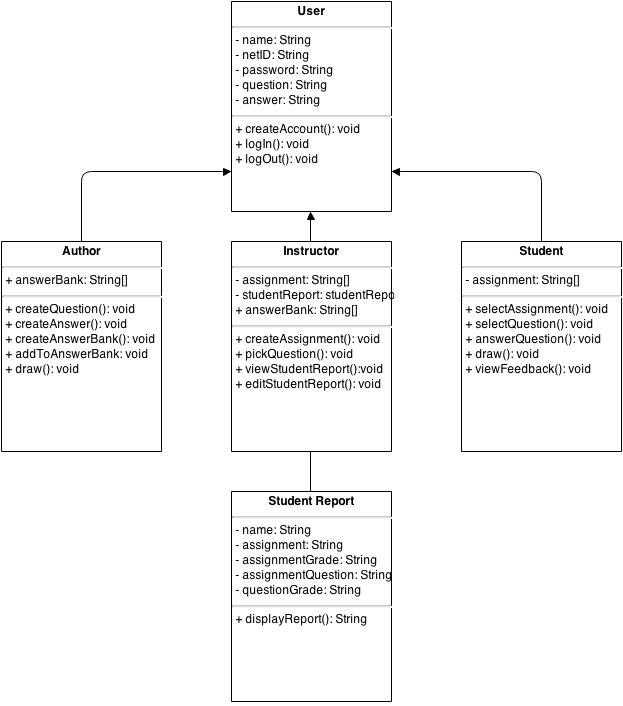
\includegraphics[height=9cm, width=12cm]{UML_1.jpg}}
            \caption{UML Diagram}
    \end{figure}

%%%%%%%%%%%%%%%%%%%%%%%%%%%%%%%%%%%%%%%%%%%%%%%%%%%%%%%%%%%
%%%%%%%%%%%%%%%%%%%%%UML%%%%%%%%%%%%%%%%%%%%%%%%%%%%%%%%%%%
%%%%%%%%%%%%%%%%%%%%%%%%%%%%%%%%%%%%%%%%%%%%%%%%%%%%%%%%%%%








\chapter{User}

User module provides a way to retrieve user’s information. It handles logging in, logging out and user registration.\\
\textbf{Interface Specifications:}\\
\begin{itemize}
    \item void create account()- Creates account, using user's input. Create a new database entry with user's ID, account type, name/email/password etc.
   \item  void logIn()- read user's input authentication input and create a new session.  
\item  void logOut()- finish user's session.
\end{itemize}
\textbf{Assumptions:}
\begin{itemize}
\item None
\end{itemize}
\textbf{Dependencies:}
Students, Instructors, Authors depend on User Module\\
\textbf{Internal Structure:}
    \begin{itemize}
      \item \textbf{Internal Methods:}
            \begin{itemize}
                \item void connectToUserDatabase()- Handles database connection.
                \item void checkNetIDUnique()- Check whether given ID does not exist in database upon registration.
            \end{itemize}
       \item \textbf{Internal Variables:}
        \begin{itemize}
            \item  name: String
            \item  netID: String
            \item  password: String
        \end{itemize}
        \end{itemize}
         \textbf{Hidden Information:}
        \begin{itemize}
        \item None
        \end{itemize}
   






\chapter{Student}
\textbf{Descrioption:} Student Module manages student's account. It handles the access to the assignment list\\
\textbf{Interface Specifications:}
\begin{itemize}
   \item void selectAssignment()- reads user's input to obtain assignment ID and then retrieves assignment from database
    \item void displayQuestion()- outputs question based on its ID
    \item void selectQuestion()- reads user's input to obtain question ID and then retrieves assignment from database
    \item void answerQuestion()- handles the input provided by Student
    \item void draw()- handles the input provided by user on the drawing board
    \item void viewFeedback()- outputs feedback based on the student's answer
\end{itemize}
\textbf{Assumptions:}
\begin{itemize}
    \item Logging in is handled by User Module
    \item Account type is provided.
\end{itemize}
\textbf{Dependencies:}
\begin{itemize}
    \item Depends on Draw
    \item Assignment
    \item Question Modules.
\end{itemize}
\textbf{Internal Structure:}
\begin{itemize}         
   \item \textbf{Internal Methods:}
           \begin{itemize}
           \item None
           \end{itemize}  
          \item  \textbf{Internal Variables:}
                  \begin{itemize}
            \item assignment: String[]
        \end{itemize}
        \end{itemize}
     \textbf{Hidden Information:}
    \begin{itemize}
    \item None
    \end{itemize}



 

\chapter{Instructor}
\textbf{Description:}Instructor module manages instructor’s account. It provides interface to create new assignments, add questions to individual assignments, make lists of students that can access a particular assignment and finally to check student report.\\
\textbf{Interface Specifications:}
\begin{itemize}
     \item   void createAssignment(): handler for creating a new assignment, reading assignment name and list of students that instructor provides, and creating list of questions
    \item    void viewStudentReport(): accesses the scores database and outputs the data upon instructors request
    \item     void editStudentReport(): instructor can update student scores and information
\end{itemize}
\textbf{Assumptions:}
\begin{itemize}
\item Depends on assignment and question, and drawing tool modules
\end{itemize}
\textbf{Dependencies:}
Students, Instructors, Authors depend on User Module\\
\textbf{Internal Structure:}
\begin{itemize}
 \item       \textbf{Internal Methods:}
\begin{itemize}
    \item void makeStudentList(): instructor makes a list of students for each assignment
    \item void makeQuestionList(): instructor makes a list of questions for each assignment
    \end{itemize}
       \item  \textbf{Internal Variables:}
\begin{itemize}
\item assignment: String[]
 \item studentReport: studentReport
 \item answerBank: String[]
\end{itemize}
 \end{itemize}
\textbf{Hidden Information:}
\begin{itemize}
\item None
\end{itemize}
 
 
\chapter{Author}
\textbf{Description: }Author module manages author's account. It provides interface to create new questions, add possible answers and feedback to individual question.\\
\textbf{Interface Specifications:}
\begin{itemize}
    \item void createQuestion(): provides interface to make a new question, with question text/diagram options/feedback, uses create answer and create feedback
    \item void draw(): provides an interface to draw a possible answer, gives an option whether to draw.
    \end{itemize}
\textbf{Assumptions:}
\begin{itemize}
\item Logging in is handled by User Module, and account type is provided.
\end{itemize}
\textbf{Dependencies:}
Depends on assignment and question, and drawing tool modules \\
\textbf{Internal Structure:}
\begin{itemize}
\item          \textbf{Internal Methods:}
\begin{itemize}
    \item void createAnswer(): reads the input provided by author in a form of diagram of text
    \item void createFeeback(): provides a way to create feedback for a created question
\end{itemize}
     \item     \textbf{Internal Variables:}
     \begin{itemize}
 \item answerBank: String[]
 \end{itemize}
 \end{itemize}
\textbf{Hidden Information:}
\begin{itemize}
\item None
\end{itemize}


%%%%%%%%%%%%%%%%%%%%%%%%%%%%%%%%%%%%%%%%%%%%%%%%%%%%%%%%%%%
%%%%%%%%%%%%%%%%%%%%%UML%%%%%%%%%%%%%%%%%%%%%%%%%%%%%%%%%%%
%%%%%%%%%%%%%%%%%%%%%%%%%%%%%%%%%%%%%%%%%%%%%%%%%%%%%%%%%%%

\chapter{UML 3}

    \begin{figure}[H]
            \centerline{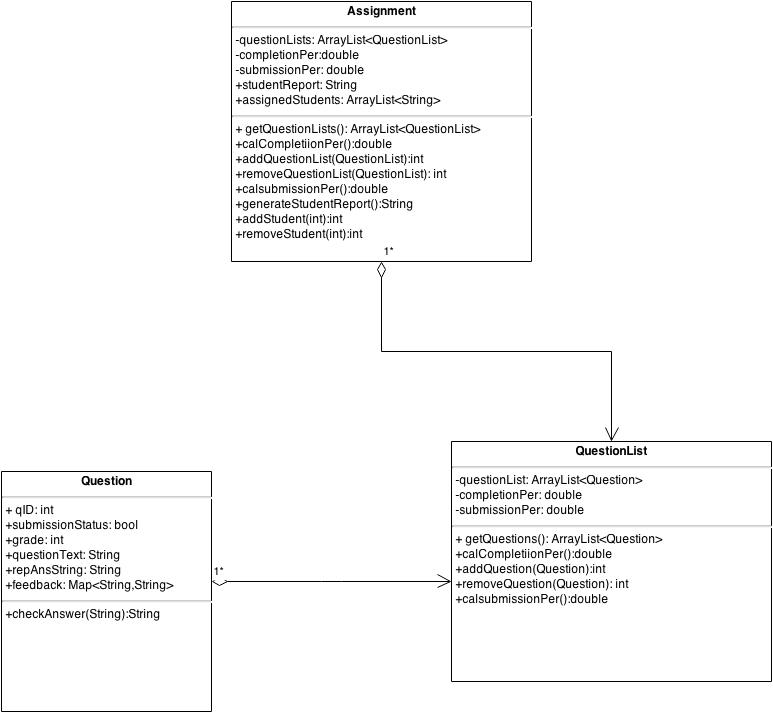
\includegraphics[height=9cm, width=10cm]{Assignment.jpg}}
            \caption{Assigments UML Diagram}
    \end{figure}

%%%%%%%%%%%%%%%%%%%%%%%%%%%%%%%%%%%%%%%%%%%%%%%%%%%%%%%%%%%
%%%%%%%%%%%%%%%%%%%%%UML%%%%%%%%%%%%%%%%%%%%%%%%%%%%%%%%%%%
%%%%%%%%%%%%%%%%%%%%%%%%%%%%%%%%%%%%%%%%%%%%%%%%%%%%%%%%%%%



\chapter{Assignment}

\textbf{Description: }An instructor creates an assignment so that the instructor can add questions or question list to the assignment. Controls what the final assignment looks like before being assigned.\\
\textbf{Interface Specifications:}
\begin{itemize}
\item void intialize(String Name) - Initialize an assignment with a specific name.
\item void addQuestion(Question) - Add a question that is in the database to the assignment. Checks to see if ''Question'' is in the database. 
\item void removeQuestion(Question) - Delete a specific question that is part of the assignment Checks to see if ''Question'' is the Question list.
\item int count() - Counts the number of questions.
\item boolean isQuestionInDB(Question) - Checks if the question is in the question database
\end{itemize}
\textbf{Assumption:}
\begin{itemize}
\item None 
\end{itemize}
\textbf{Dependencies:} None \\
\textbf{Internal Structure:}
\begin{itemize}
\item \textbf{Internal Methods:}
\begin{itemize}
\item	void addList(questionList) - Add a list of questions to the assignment.
\item void removeList(questionList) - Deletes the list of questions from the assignment. Checks to see if the list is in the assignment.
\item void saveAssignment() - Save assignment to the assignment database
\item	String getName() - returns name of the assignment
\item	void changeName() - changes the name of the assignment
\end{itemize}
\item \textbf{Internal Variables:}
\begin{itemize}
\item	ArrayList[] Question
\item	String Name
\item	int count
\end{itemize}
\end{itemize}
\textbf{Hidden Information:}
\begin{itemize}
\item None
\end{itemize}



\chapter{Question List}

\textbf{Description: }It's a list of questions from which an instructor can choose to add the list to an assignment or view the list and then view individual questions. This list is used for a student to pick and choose which questions to answer in a specific assignment. \\ 
\textbf{Interface Specifications:}
\begin{itemize}
\item void initialize() - Initialize a list for questions to be added in the future. This list can be added to assignments. This is called when an instructor wants to make a question list.

\item void addQuestion(Question) - Add a question that is in the database to the question list. Checks to see if ''Question'' is in the database. 

\item void removeQuestion(Question) - Delete a specific question that is part of the question list. Checks to see if ''Question'' is the Question list.

\item int count() - Counts the number of questions.

\item boolean isQuestionInDB(Question) - Checks if the question is in the question database
\end{itemize}
\textbf{Assumptions:}
\begin{itemize}
\item None
\end{itemize}
\textbf{Dependencies:} None \\
\textbf{Internal Structure}
\begin{itemize}
\item	\textbf{Internal Methods}
\begin{itemize}
	\item boolean isEmpty() - Checks if the list is empty
	\item void find(Question) - Searches for the question in the list
\end{itemize}
	\item \textbf{Internal Variables}
	\begin{itemize}
        \item ArrayList[] Questions;
	    \item int count;
    \end{itemize}
\end{itemize}
\textbf{Hidden Information:}
\begin{itemize}
\item None
\end{itemize}



\chapter{Question}

\textbf{Description: }Questions can be made by the author. These questions will be added to the database and can be copied from the database and used for question list and assignments.\\
\textbf{Interface Specifications:}
\begin{itemize}
    \item void addQuestion(Question) - adds the question to the database.
    \item void removeQuestion(Question) - remove question from database.
    \item boolean isQuestionInDB(Question) - Checks if the question is in the question database
\end{itemize}
\textbf{Assumption:}
\begin{itemize}
\item An Answer will be provided with the question.
\end{itemize}
\textbf{Dependencies:} None \\
\textbf{Internal Structure:}
\begin{itemize}
	\item \textbf{Internal Methods:}
	\begin{itemize}
	\item Question makeQuestion(String Name); Makes a question to be added to the database
of questions.
    \item Diagram drawAnswer(); Make an answer to be assigned with this question.
    \item void UpdateQuestion(); Updates the question, adds question to database
    \end{itemize}
\item 	\textbf{Internal Variables:}
	\begin{itemize}
	\item String Name;
	\item Diagram Answer;
	\item String Question;
	\end{itemize}
\end{itemize}
\textbf{Hidden Information:}
\begin{itemize}
\item None
\end{itemize}





















%%%%%%%%%%%%%%%%%%%%%%%%%%%%%%%%%%%%%%%%%%%%
\chapter{Validator}
\textbf{Description:}
This module is responsible for validating a diagram provided by a student. compares it to the correct diagram created by the author which it retrieves from the database. Because there are multiple variations of the same diagram available, we also need to make sure to compare these variations to the correct diagram. \\
\textbf{Interface Specification:}
    \begin{itemize}
            	\item diagram getCorrectDiagram(int): retrieves the solution from the database given question ID
            \item	boolean validateSolution(diagram, diagram): compares input diagram and correct diagram and outputs whether they are equivalent
    \item 	void sendFeedback(): send feedback provided by the author
    String\\
    \item getFeedback(int): retrieve feedback for a given question from database
    \item void updateReport(): update student report given the result of comparison of student’s input with the correct diagram
\end{itemize}
 \textbf{Assumptions:}
 \begin{itemize}
        \item 	We are assuming that the correct answer for the diagram is in database and that the input comes in JSON format
\end{itemize}
\textbf{Dependencies:}

        	This module depends on the Serializer and DBAccessor modules \\
\textbf{Internal Structure:}
\begin{itemize}
\item\textbf{Internal Methods:}
\begin{itemize}
    \item  String[] constructAllVariation(diagram): make all possible variations of JSON strings corresponding to input diagram
\textbf{Internal Variables:}
               \end{itemize}
\item\textbf{Internal Variables:}
\begin{itemize}
\item {None}
\end{itemize}
\end{itemize}
\textbf{Hidden Information:}
\begin{itemize}
\item {None}
\end{itemize}
        	
 
\chapter{DBAccessor}
\textbf{Description:}
This module is responsible for retrieving required information from the database such as user information, diagram and questions. \\
\textbf{Interface Specification:}
\begin{itemize}
\item        	String getQuestion(int): retrieves question information from database provided
ID of the question
\item	void addQuestion(question): adds question to the database
\item	void editQuestion(): edit questions
        \item	String getAssignment(int): retrieves assignment information from database provided ID of the assignment
\item	void addAssignment(): adds assignment to the database
	\item void editAssignmnet(): edit assignment
        \item 	String getSolution(int): retrieves JSON string pf the correct solution given question ID
        \item 	String getUserInfo(int): retrieve all the information about the USER given his ID
	\item String getFeedback(int): retrieves feedback provided by the author given the question ID
	\item void updateFeedback(String, int): update or create new feedback given question ID
        \item 	void getUserInfo(): retrieve user’s information such as name, ID etc
\item 	void addUserInfo() create a new entry in user database
\item 	void removeQuestion(int): removes question from the database given question ID
\item 	void removeAssignment(): removes assignment from database
\item 	void getStudentReport(): retrieves student report from
the database\\
\end{itemize}
\textbf{Assumptions:}
\begin{itemize}
        \item	Correct name and password of the database are provided for this module
        \end{itemize}
\textbf{Dependencies:}
        	This module depends on all modules using the database: User, Validator\\
\textbf{Internal Structure:}
\begin{itemize}
\item \textbf{Internal Methods:}
\begin{itemize}
\item                    	void connectToDatabase(): establishes a connection to database using name and password provided
\end{itemize}
\item \textbf{Internal Variables:}
\begin{itemize}
\item                    	String databaseName: stores database name
     \item   	        	String databasePassword: store the database password
 \end{itemize}
\end{itemize}
\textbf{Hidden Information:}
\begin{itemize}
\item None
\end{itemize}





\end{document}
